\begin{figure*}
    \centering
    \subfigure[\citeauthor{Gionis2007}(\citeyear{Gionis2007})中的测试结果. \label{fig:3a}]{
        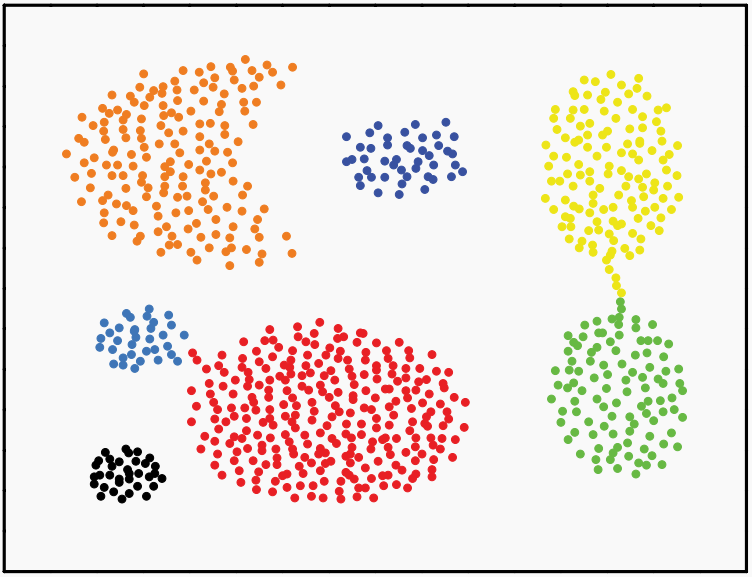
\includegraphics[scale=.2]{3_a.png}
    }\ 
    \subfigure[\citeauthor{Fraenti2006}(\citeyear{Fraenti2006})中的测试结果. \label{fig:3b}]{
        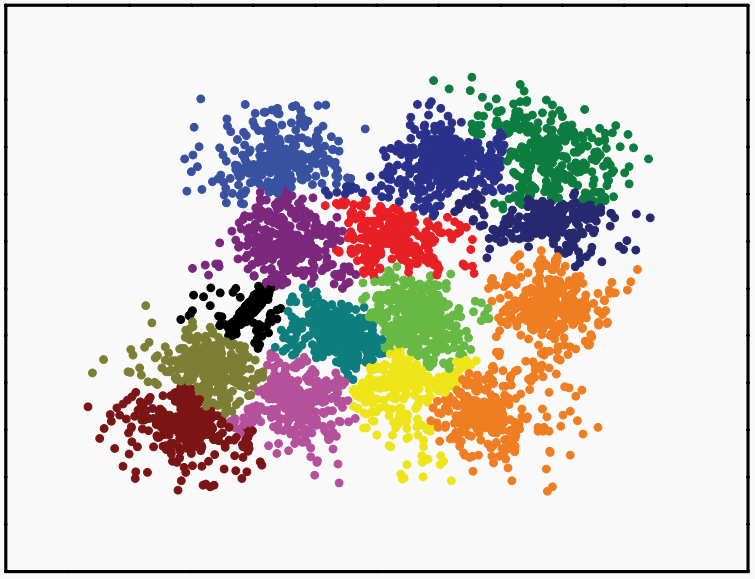
\includegraphics[scale=.2]{3_b.png}
    }\\
    \subfigure[\citeauthor{{Fu2007}}(\citeyear{Fu2007})中的测试结果. \label{fig:3c}]{
        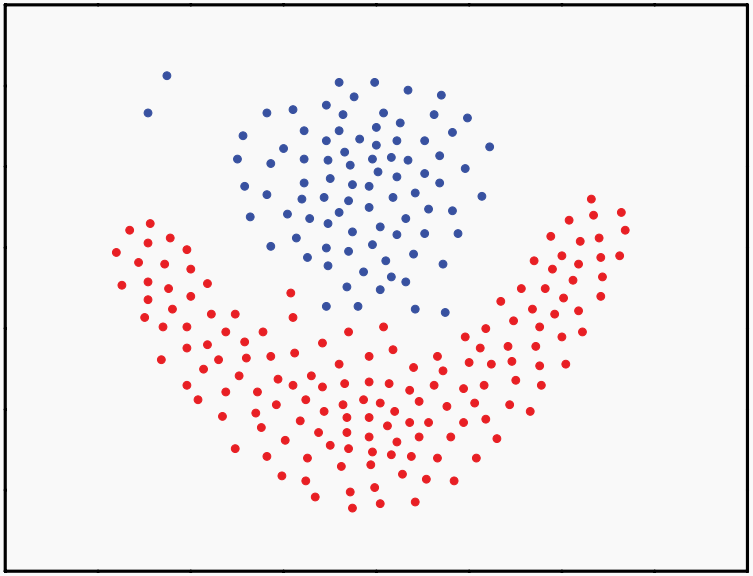
\includegraphics[scale=.2]{3_c.png}
    }\ 
    \subfigure[\citeauthor{{Chang2008}}(\citeyear{Chang2008})中的测试结果. \label{fig:3d}]{
        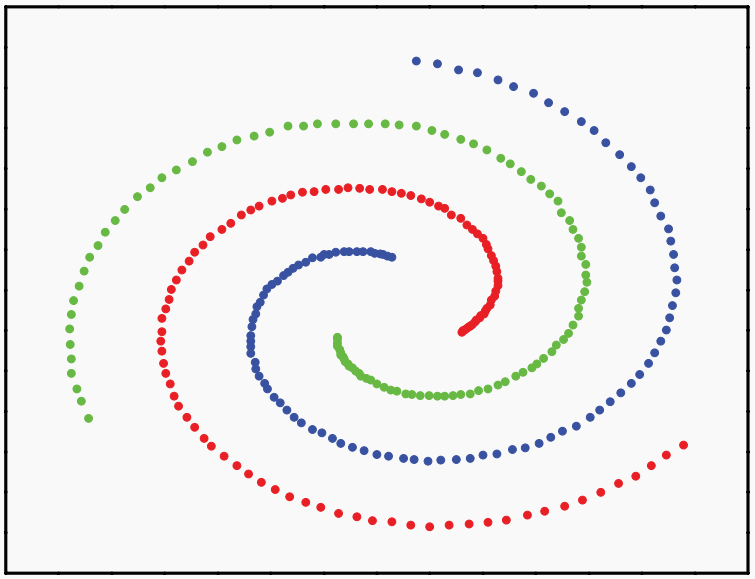
\includegraphics[scale=.2]{3_d.png}
    }
    \caption{其他文献中测试例子的结果. \label{fig:3}}
\end{figure*}

为了测试此算法, 我们首先考虑图~\ref{fig:2} 中的例子, 其数据是从一个具有非球形和剧烈重叠的概率分布中抽取的(图~\ref{fig:2a}). 图~\ref{fig:2b}、\ref{sub@fig:2c}是, 分别从图~\ref{fig:2a} 中中抽取的4000和1000个点, 在相应的决策图(图~\ref{fig:2d}, \ref{sub@fig:2e})中, 只看到5个点的$\sigma$值很大, 密度也相当大. 这些点在图中表示为大的实心圆, 对应于聚类中心. 选定聚类中心后, 每个点要么被分配到一个簇, 要么被分配到环, 即使是对那些密度非常不同的(图~\ref{fig:2c} 中的蓝色和浅绿色点)和非球形峰, 该算法也可以捕捉到概率分布的位置和形状. 此外, 通过目测图~\ref{fig:2a} 中的概率分布可以知道, 分配到环的点对应的区域不会被分到任何类中. 

为了表明该算法对大量数据也具有鲁棒性, 我们从图~\ref{fig:2a} 中抽取10000个点进行分析, 将从10000个样本上获得的聚类结果作为参考, 通过只保留一部分点来获得缩小的样本, 并对每个缩小的样本独立地进行聚类. 图~\ref{fig:2f} 是分配到一个簇的点的误分率与样本量的关系图像, 可以看到, 即使对只包含1000个点的小样本, 被错误分类的点占比仍然远低于$1\%$. 

对图~\ref{fig:2b} 中的数据改变$d_c$, 会产生一致的结果(图~S1 所示\footnote{类似于图~S1, S2 的图片可以在\url{http://science.sciencemag.org/content/suppl/2014/06/25/344.6191.1492.DC1}中获得. }). 
可以经验地按照如下规律选择$d_c$, 使平均邻域数约为数据量的$1\sim2\%$. 对于由少量点组成的数据集, $\rho_i$可能会受到较大的统计误差的影响. 在这些情况下, 最好用更精确的方法估计密度\cite{Fukunaga1975,Cheng1995}. 

接下来, 我们在图~\ref{fig:3} 的例子上对算法进行了测试. 对于计算点少的密度, 我们采用了\citeauthor{Cheng1995}(\citeyear{Cheng1995})中描述的指数核算法, 在图~\ref{fig:3a} 中, 我们使用了\citeauthor{Gionis2007}(\citeyear{Gionis2007})中的一个数据集, 得到的结果与原文的结果基本一致, 而文中说到许多常用的方法无法成功将此数据集聚类. 在图~\ref{fig:3b} 中, 我们使用了\citeauthor{Fraenti2006}(\citeyear{Fraenti2006})中的一个15个概率分布高度重合的例子, 我们的算法成功地确定了每个簇的结构. 在图~\ref{fig:3c} 中, 我们使用了FLAME方法\cite{Fu2007}中的例子, 得到的结果与原始方法高度一致. 在图~\ref{fig:4d} 所示的为了说明基于路径的谱聚类\cite{Chang2008}的性能而引入的数据集中, 我们的算法在不需要生成连接图的情况下, 正确地找到了三个簇. 作为比较, 在图~S3 和 S4 中, 我们展示了基于路径的谱聚类\cite{Chang2008}的性能. 图~S3和 S4 中, 我们展示了这四个测试案例和图~\ref{fig:2} 中的例子通过K-means\cite{MacQueen1967}获得的聚类结果. 在大多数情况下, 即使使用正确的K值进行K-means聚类, 也不能得到很好的结果. 

该方法对于度量的变化是稳健的, 即保持式~\ref{equ:1} 中的密度估计不变, 这些变化也不会对小于$d_c$的距离产生显著影响. 显然, 式~\ref{equ:2} 中的距离会受到这种度量变化的影响, 但决策图的结构(特别是d值大的数据点的数量)是密度值排序的结果, 而不是远处的点之间实际距离的结果, 证明这一说法的例子如图~S5 所示. 

我们的方法只需要测量(或计算)所有数据点之间的距离, 而不需要对概率分布\cite{McLachlan2007}或多维密度函数\cite{Fukunaga1975}进行参数化. 因此, 其性能不受数据点所嵌入的空间的内在维度影响. 同时, 我们还验证了在256个维度\cite{Franti2006}的16个聚类的例子中, 该算法可以找到正确的聚类中心的数量, 并正确的将数据点划分到每一个簇中(图~S6). 对于\cite{Charytanowicz2010}中三类小麦种子的7个X射线特征的210个测量数据, 该算法正确预测了3个簇的存在, 并对$97\%$的数据进行了正确分类(图~S7, S8). 

\begin{figure*}
    \centering
    \subfigure[数据库中前一百张图片的决策图\cite{Samaria1994}. \label{fig:4a}]{
        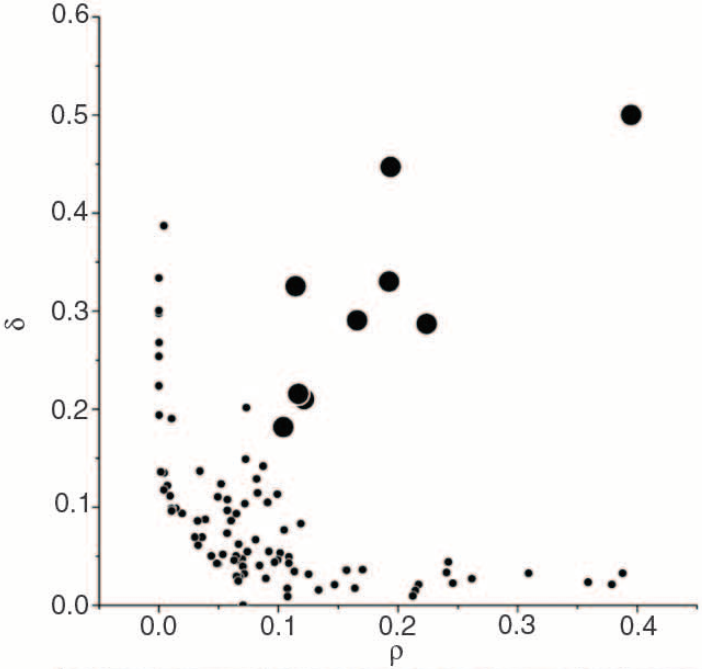
\includegraphics[scale=.15]{4_a.png}
    }\ 
    \subfigure[$\gamma_i=\rho_i\sigma_i$, 其值依次递减. \label{fig:4b}]{
        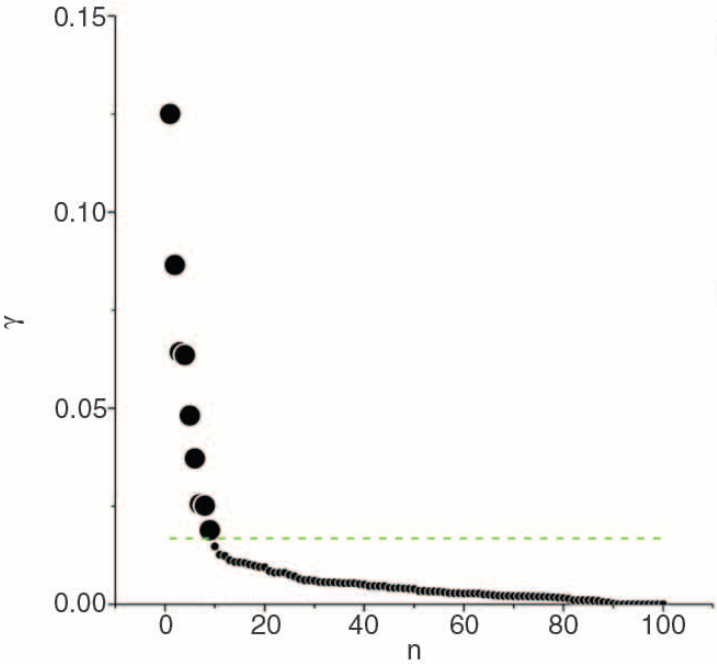
\includegraphics[scale=.15]{4_b.png}
    }\ 
    \subfigure[性能曲线. \label{fig:4c}]{
        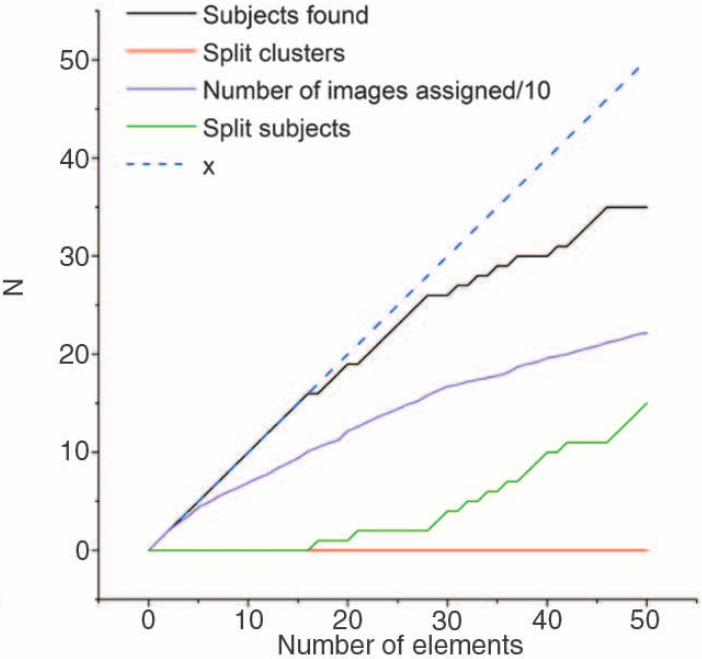
\includegraphics[scale=.15]{4_c.png}
    }\\
    \subfigure[前100张图像的聚类结果的图示. 具有相同颜色的面孔属于同一簇, 聚类中心用白色圆圈标注.  \label{fig:4d}]{
        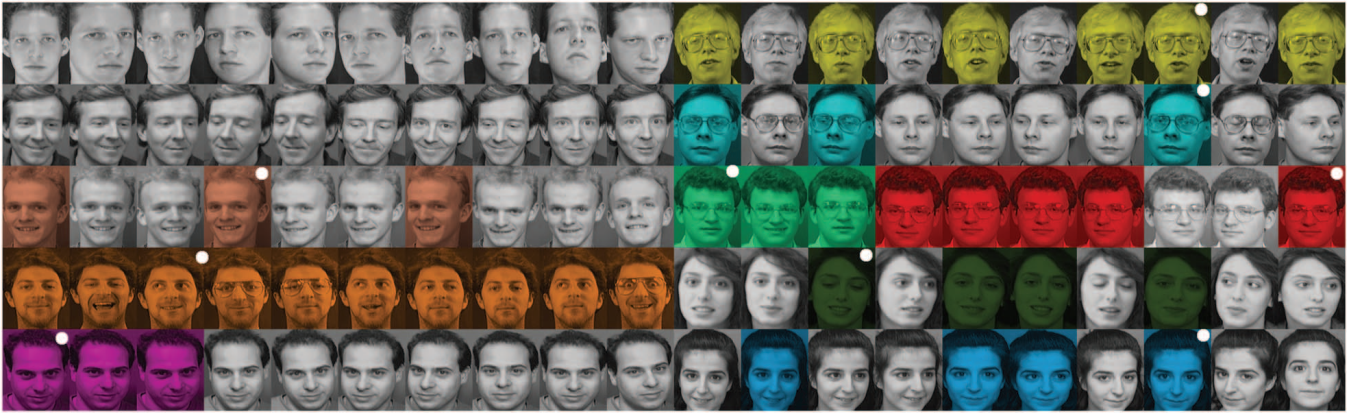
\includegraphics[scale=.25]{4_d.png}
    }
    \caption{Olivetti人脸数据库上的聚类分析. \ref{sub@fig:4c} 中, 黑线是被识别为人像的数量, 红线是包含超过一个人像的簇数, 绿线是在簇中分裂的人物数量, 紫线是划分给一个簇的图像数量除以10. \label{fig:4}}
\end{figure*}

我们还将该方法应用于Olivetti人脸数据库\cite{Samaria1994}, 这是机器学习算法的一个较为普遍的测试数据及, 使用这个数据集的目的是在没有任何先前训练的情况下, 希望算法能够识别数据中的不同的人的数量. 这个数据集对我们的方法提出了严峻的挑战, 因为``理想"的聚类中心数量与数据集中的样本数量相同, 这使得对密度的估计变得困难. 两幅图像之间的相似度是通过\cite{Sampat2009}中的方法计算的, 密度是由一个方差为$d_c=0.07$的高斯核\cite{Cheng1995}估计出来的. 对于这样一个小的集合, 密度估计器不可避免地会产生较大的误差, 因此, 我们对于数据点的划分应该更严格一些. 只有当一个图像的距离小于$d_c$时, 它才会被分配到与其最近的密度较高的图像的同一簇中. 因此, 距离任何其他密度较高的图像比dc更远的图像会不被分配. 在图~\ref{fig:4} 中, 我们显示了对数据集中前100张图像进行分析的结果. 决策图(图~\ref{fig:4a})显示了几个不同的密度最大值的存在. 与其他例子不同的是, 它们的确切数量并不清楚, 这是因为数据比较稀疏性的结果, 按递减顺序排列的$\gamma_i = \rho_i\sigma_i$图提供了一个选择聚类中心数量的提示(图~\ref{fig:4b}), 这张图显示, 聚类中心的数量比较多, 从第九个数据点开始异常增长, 因此, 我们使用9个聚类中心来进行分析. 在图~\ref{fig:4d} 中, 我们用不同的颜色显示了这些中心对应的聚类. 7个类对应不同的主体, 表明算法能够 ``识别"10个人物中的7个, 第8个被划分到了两个不同的类中. 当对数据中的所有400张图像进行分析时, 决策图不能清楚地识别出聚类的数量(图~S9). 然而, 在图~\ref{fig:4c} 中, 可以看出通过增加聚类中心, 大约有30个人物可以被毫不含糊地识别出来(图~S9), 当加入更多的中心时, 一些人物的图像会被划分到两个簇内, 但所有的簇仍然是一致的, 即只包括同一人物的图像. 按照\citeauthor{Dueck2007}(\citeyear{Dueck2007})的方法, 我们还计算了同一人物的图像被正确划分到同一簇的比率($r_{\mathrm{true}}$)和不同人物的图像被错误地分配到同一簇的比率($r_{\mathrm{false}}$). 如果在划分中不应用$d_c$处的截止值(即应用我们算法的一般公式), 则在约42到约50个中心的情况下, 可以得到$r_{\mathrm{true}}\sim 68\%$和$r_{\mathrm{false}}\sim 1.2\%$, 这一性能与无监督图像分类的最先进方法相当\cite{Dueck2007}. 

最后, 我们对聚类算法进行了基准分析, 在300K的水\cite{Marinelli2009}中对三丙氨酸的分子动力学轨迹进行了分析, 这种情况下, 聚类将近似对应于动力学盆地, 即长时间上稳定的和且被自由能量壁垒隔绝的系统独立构象, 只有在微观时间尺度上偶尔跨越. 我们首先通过标准方法\cite{Horenko2006}, 基于动力学矩阵的谱分析对轨迹进行了分析, 其矩阵特征值与系统的松弛时间有关. 在第七个特征值(图~S10)之后存在一个空隙, 表明该系统有八个盆地, 与此相一致, 我们的聚类分析(图~S10)也产生了八个聚类, 这与动力学盆地的构象一一对应\cite{Horenko2006}. 

识别具有密度最大值的聚类是一个简单而直观的选择, 就像这里和其它基于密度的聚类算法\cite{Ester1996,Fukunaga1975}所做的那样, 但这种方法有一个重要的缺点, 如果随机生成数据点, 那么对于有限样本量所估计的密度远远不是均匀的, 而是以几个最大值为特征. 然而, 决策图允许我们将真正的聚类与噪声产生的密度波纹区分开来. 定量来看, 只有在前一种情况下, 对应于聚类中心的点与其它点在$\rho$和$\sigma$上有相当大的差距, 对于随机分布, 人们反而会观察到$\rho$和$\sigma$的连续分布. 事实上, 我们对超立方体中的均匀分布随机生成的点进行了分析, 在式~\ref{equ:1}和\ref{equ:2}的点之间的距离是在超立方体上的周期性边界条件下计算出来的, 这一分析表明, 对于随机分布的数据点, 数量$\gamma_i= \rho_i\sigma_i$是按照幂律分布的, 其指数取决于点所在空间的维度. 对于实际的数据集, 如图~\ref{fig:2}至图~\ref{fig:4}中的数据集, $\gamma$的分布与幂律有明显的不同, 特别是在高$\gamma$的区域(图~S11)上. 这一结果可以为自动选择聚类中心的提供标准以及在统计学上对我们的算法的验证的可靠性提供依据. 

